\documentclass[pdf]{beamer}
\mode<presentation>{}

\usepackage[utf8]{inputenc}
\usepackage[english,serbian]{babel}

\usetheme{Madrid}
\useoutertheme{miniframes}
\useinnertheme{circles}


\title{Etika u računarstvu}
\subtitle{Seminarski rad}% u okviru kursa\\Metodologija stručnog i naučnog rada\\ Matematički fakultet}
\author[]{Marina Borozan, Matija Miličević,\\
	Stefan Mirić, Nikola Vuković}

\begin{document}

\begin{frame}
	\titlepage
	\end{frame}


\begin{frame}
\frametitle{Uvod}

\begin{itemize}
\item{Tehnološki razvoj i nove mogućnosti}
\item{Ubrzane promene u računarstvu}
\item{Moralne dileme i prihvatanje odgovornosti}
\item{Kratak sadržaj:}
	\begin{itemize}
	\item{Uvod u teoriju etike}
	\item{Etika u računarstvu}
	\item{Razvoj tehnologije i primena etike}
	\end{itemize}
\end{itemize}

\end{frame}
\begin{frame}
\frametitle{Etika}

Oblast filozofije koja se bavi sistematizacijom, odbranom i preporukom ispravnog i pogrešnog ponašanja



\begin{itemize}
\item{Metaetika}
	\begin{itemize}
	\item[--]{Bavi se temeljima etike i apstraktnim pitanjima}
	\end{itemize}
\item{Normativna etika}
	\begin{itemize}
	\item[--]{Najkorisnija za temu etike u računarstvu}
	\item[--]{Definiše konkretne načine sagledavanja moralnih pitanja}
	\end{itemize}
\item{Primenjena etika}
	\begin{itemize}
	\item[--]{Razmatra konkretne situacije i moralna pitanja}
	\item[--]{Primenjuje principe definisane u normativnoj etici}
	\end{itemize}
\end{itemize}

\end{frame}

\begin{frame}
\frametitle{Teorije etike}

\begin{itemize}
\item{Pojam dobrog}
\item{Pojam ispravnog}
\end{itemize}

\begin{table}
\begin{center}
\begin{tabular}{|l|c|c|c|} \hline
Teorija & Etika vrline & Deontologija & Konsekvencijalizam\\ \hline
Fokus & Delatnik & Delo & Posledice\\ \hline
Predstavnik & Aristotel & Imanuel Kant & Džon Stjuart Mil\\
& 384-322 PNE & 1724-1804 & 1806-1873\\ 
& 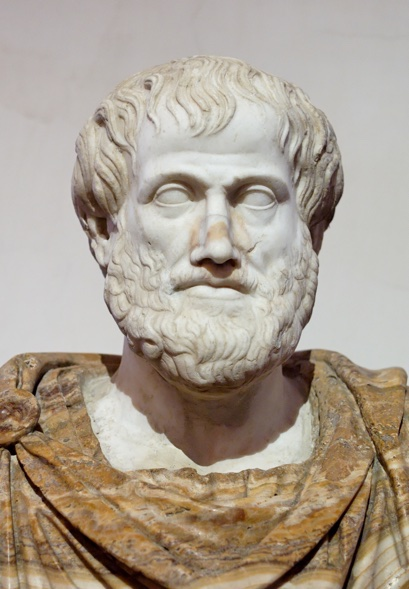
\includegraphics[scale=.1]{slike/aristotel.jpg} & 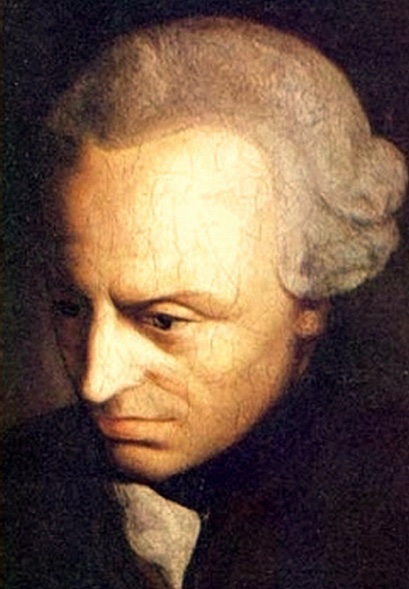
\includegraphics[scale=.1]{slike/kant.jpg} & 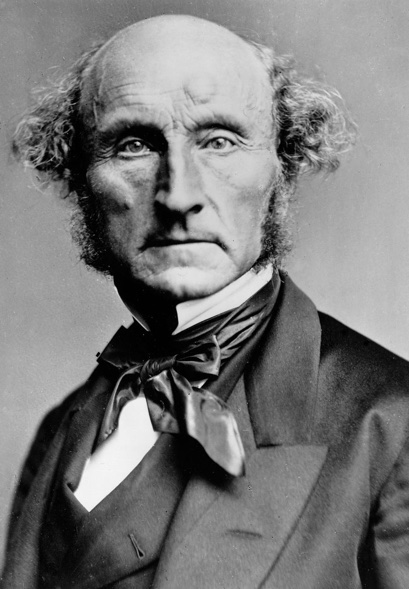
\includegraphics[scale=.1]{slike/mil.jpg} \\
\hline
\end{tabular}
\label{tab:tabela1}
\caption{{Pregled teorija etike i vrednosti koje zastupaju}}
\end{center}
\end{table}

\end{frame}

\begin{frame}
\frametitle{Deontologija}

\begin{itemize}
\item{Dužnost (deon) i nauku (logos)}
\item{Procenjuje moralnost postupaka}
\end{itemize}
\textbf{Kantijanizam}
\begin{itemize}
\item{Najpoznatija podgrana deontologije}
\item{Principi:}
	\begin{itemize}
	\item[--]{Univerzalnost moralnih zakona}
	\item[--]{Dobra volja kao motiv}
	\item[--]{Pojam \textcolor{purple}{dužnosti}} 
	\end{itemize}
\item{Kategorički imperativ:\newline
I: ``Postupaj prema onoj maksimi za koju možeš poželeti da postane opšti zakon.''\newline
II: ``Postupaj prema ljudskosti u sebi i u drugim bićima uvek kao prema cilju, a nikad kao prema sredstvu.''}
\end{itemize} 

\end{frame}
\begin{frame}
\frametitle{Konsekvencijalizam}

\textbf{Konsekvencijalizam}\newline
Procenjuju se posledice i krajnji ishodi moralnih izbora
\begin{itemize}
\item{\textbf{Utilitarizam postupaka}}
	\begin{itemize}
	\item[--]{Vrednuje samo direktne posledice dela}
	\item[--]{Suma pozitivnih i negativnih posledica}
	\end{itemize}
\item{\textbf{Utilitarizam pravila}}
	\begin{itemize}
	\item[--]{Vrednuje pravila po posledicama do kojih dovodi njihovo pridržavanje}
	\item[--]{Generalizacija dela u pravilo}
	\end{itemize}
\end{itemize}


\end{frame}
\begin{frame}
\frametitle{Etika vrline}

\textbf{Etika vrline}
\begin{itemize}
\item{Pojmovi ključni za moralan život - edukacija, mudrost, društvene veze, uloga emocija...}
\item{Pojam \textcolor{purple}{vrline}}
\item{Moralni izbori se definišu kao izbori moralnih osoba}
\item{Poroci - suprotni vrlinama}
\end{itemize}

\end{frame}


\begin{frame}
\frametitle{Etika i tehnološki razvoj}

	Nove tehnologije:

	\begin{itemize}

	\item Nove mogućnosti

	\item Novi problemi

	\end{itemize}

	Stavovi o tehnološkom napretku:

	\begin{enumerate}

	\item Tehnicizam - tehnologija je koristan alat za ljudsko društvo
	\item Optimizam - tehnologija je moralno dobra
	\item Skepticizam - postoje ozbiljni rizici pri tehnološkom napretku

	\end{enumerate}

	\end{frame}


\begin{frame}
\frametitle{Računarska Etika}
	
	Kratka istorija:
	\begin{itemize}
	
	\item Norbert Viner
	\begin{itemize}
	\item[--] ``Kibernetika'' (1948)
	\item[--] ``Ljudska upotreba ljudskih bića'' (1950)
	\end{itemize}
	
	\item Volter Maner
	\begin{itemize}
	\item[--] Eksperimentalni kurs (1976)
	\item[--] Plan kursa (1978)	
	\item[--] Monograf (1980)
	\end{itemize}
	\end{itemize}
	\end{frame}

\begin{frame}
\frametitle{Viđenja Računarske Etike}

	\begin{itemize}

	\item Džejms Mur: ``Šta je računarska etika?'' (1985)

	\item Debra Džonson ``Računarska etika'' (1985)
	
	\end{itemize}

	Pristupi u naučnoj literaturi:
	\begin{enumerate}
	\item Pristup nepostojanja (No resolution approach)
	\item Profesionalni pristup (The professional approach)
	\item Radikalni pristup (The radical approach)
	\item Konzervativni pristup (The conservative approach)
	\item Inovativni pristup (The innovative approach)
	\end{enumerate}
	\end{frame}


\begin{frame}
\frametitle{Preporuke etičkog postupanja}

	\begin{itemize}

	\item Sajber zločin
	
	\item Potreba za pravilima ponašanja

	\end{itemize}

	Predlozi institucija:
	\begin{itemize}
		\item Association for Computing Machinery - ACM
		\\- Kodeks etičkog i profesionalnog ponašanja (1973)
		\\ - Don Parker (SRI International) - vođa odbora
		\item The Computer Ethics Institute - CEI
		\\- 10 zapovesti računarske etike (1992)
	\end{itemize}


\end{frame}


\begin{frame}
\frametitle{Primeri etičkih dilema u računarstvu}
		Pisanje virusa:
		\begin{itemize}
		\item Kalgari Univerzitet (Ken Barker)
			\begin{itemize}
			\item Pisanje virusa na kursu računarske sigurnosti
			\item Zabrinutost antivirusnih kompanija 
			\end{itemize}
		
		\item Sonoma Univerzitet (Džordž Ledin)
			\begin{itemize}
			\item Osnovao kurs za pravljenje bolje sigurnosne zaštite
			\item Bojkot sigurnosnih kompanija
			\end{itemize}
		\end{itemize}
\end{frame}


\begin{frame}
\frametitle{Primeri etičkih dilema u računarstvu}
	Neki dodatni primeri:
	\begin{itemize}
	\item Da li je prihvatljivo da se kupi softver pa onda instalirati ga dvaput?
	\item Šta ako ga instaliramo, a zatim napravimo 50 kopija i prodamo zainteresovanim kupcima?
	\item Da li kompanija ima pravo da čita elektronsku poštu svojih zaposlenih?
	\item Da li kompanija ima pravo da nadzire koje Web stranice njeni zaposleni posećuju?
	\item Da li korisnik ne sme da modifikuje program iako je njegov cilj da ga poboljša?
	\end{itemize}
\end{frame}

\begin{frame}
\frametitle{Zaključak} %TODO Zaključak, kraj, rezime?

%TODO stvarno ne znam šta bih stavio ovde

	Rezime:

	\begin{itemize}	
	\item Motivacija izučavanja računarske etike	
	\item Metodologije %računarske etike
	\item Društvena korist %računarske etike
	\end{itemize}

Hvala na pažnji!

\end{frame}

\begin{frame}
\frametitle{Literatura}

	\begin{itemize}	
	\item Michael J. Quinn - \textcolor{blue}{Ethics for the information age} - 7th edition, Pearson, 2017
	\item James Fieser - \textcolor{blue}{Ethics} - Internet Encyclopedia of Philosophy
	\item Kevin M. DeLapp - \textcolor{blue}{Metaethics} - Internet Encyclopedia of Philosophy
	\item Larry Alexander, Michael Moore - \textcolor{blue}{Deontological Ethics}, 2015
	\item Terrell W. Bynum - \textcolor{blue}{Computer and Information Ethics} - Stanford Encyclopedia of Philosophy, 2015
	\item Luciano Floridi, J.W. Sanders - \textcolor{blue}{Mapping the foundationalist debate in computer ethics} - University of Oxford
	\item \textcolor{blue}{ACM Code of Ethics and Professional Conduct} - Association for Computing Machinery, 2018
	\item \textcolor{blue}{The  Ten  Commandments  of  Computer  Ethics} - The  Computer  Ethics  Institute
	\end{itemize}



\end{frame}

\end{document}

